\documentclass[conference]{IEEEtran}
\IEEEoverridecommandlockouts

\usepackage{cite}
\usepackage{amsmath,amssymb,amsfonts}
\usepackage{algorithmic}
\usepackage{algorithm}
\usepackage{graphicx}
\usepackage{textcomp}
\usepackage{xcolor}
\usepackage{booktabs}
\usepackage{microtype}
\usepackage{tabularx}
\usepackage{multirow}
\usepackage{url}
\usepackage{balance}

% Correct bad hyphenation here
\hyphenation{op-ti-cal net-works semi-conduc-tor Mind-Bridge psy-cho-met-ric}

\begin{document}

\title{MindBridge: An AI-Augmented Non-Clinical Surveillance, Standardized Assessment, and Well-being Tracking Platform for Children\\
\thanks{This work was supported by the Department of Computer Science and Engineering, School of Engineering, Presidency University, Bengaluru, India.}
}

\author{
\IEEEauthorblockN{Harsha R}
\IEEEauthorblockA{\textit{Dept. of Computer Science and Engineering} \\
\textit{Presidency University}\\
Bengaluru, Karnataka, India \\
USN: 20231CSE0261}
\and
\IEEEauthorblockN{Arjun M}
\IEEEauthorblockA{\textit{Dept. of Computer Science and Engineering} \\
\textit{Presidency University}\\
Bengaluru, Karnataka, India \\
USN: 20231CSE0277}
\and
\IEEEauthorblockN{Abhishek M R}
\IEEEauthorblockA{\textit{Dept. of Computer Science and Engineering} \\
\textit{Presidency University}\\
Bengaluru, Karnataka, India \\
USN: 20231CSE0268}
\and
\IEEEauthorblockN{Jetti Satya Sai Kumar}
\IEEEauthorblockA{\textit{Assistant Professor, Dept. of CSE} \\
\textit{Presidency University}\\
Bengaluru, Karnataka, India \\
jettisatyasaikumar@presidencyuniversity.in}
}

\maketitle

\begin{abstract}
Childhood and adolescent psychological distress often manifests subtly through daily lifestyle and behavioral shifts---including chronic sleep insufficiency, excessive sedentary screen engagement, reduced active play, and acute academic stress---long before reaching formal clinical thresholds. However, conventional pediatric mental health screening is largely episodic, adult-mediated, and confined to structured clinical or school environments that fail to capture real-time behavioral fluctuations. This paper presents \textbf{MindBridge}, an interactive, child-centered digital platform engineered for non-clinical well-being surveillance, multi-modal lifestyle tracking, standardized psychometric assessment, and emergency referral routing among individuals aged 8--17. MindBridge couples a low-cognitive-load child portal with a dual-modality inference engine: (1) a supervised Random Forest classifier trained on a domain-modeled dataset of 2,000 lifestyle records that stratifies multi-factor behavioral inputs into three non-diagnostic tiers (\textit{Low/Healthy}, \textit{Moderate/Monitoring}, and \textit{Elevated/Action Advised}); (2) a local, zero-retention Natural Language Processing (NLP) module utilizing the VADER lexicon to infer affective valence from optional journal entries strictly in-memory; and (3) an integrated digital implementation of the standardized \textbf{Pediatric Symptom Checklist (PSC-17)} evaluating Internalizing, Attention, and Externalizing subscales against clinical cutoffs. The platform is implemented across a decoupled FastAPI/SQLite backend and a responsive React~18 single-page application. Experimental evaluation via 5-fold stratified cross-validation demonstrates a classification accuracy of \textbf{77.25\% $\pm$ 1.37\%}, a weighted F1-score of \textbf{0.88}, and a critical \textbf{1.00 recall rate} on the safety-sensitive Elevated Risk tier. The architecture enforces a strict privacy-by-design model in compliance with Section~9 of India's Digital Personal Data Protection (DPDP) Act, 2023.
\end{abstract}

\begin{IEEEkeywords}
Pediatric Well-being, Mental Health Surveillance, Digital Health Informatics, Pediatric Symptom Checklist (PSC-17), Random Forest, VADER Sentiment Analysis, Privacy-by-Design, DPDP Act 2023.
\end{IEEEkeywords}

\section{Introduction}
\label{sec:intro}
The global escalation of mental health challenges among children and adolescents has emerged as a significant public health issue. Epidemiological data published by the World Health Organization (WHO) indicates that approximately 14\% (1 in 7) of individuals aged 10--19 experience a diagnosable mental disorder, with suicide representing the fourth leading cause of death among older adolescents worldwide \cite{who2022mental, unicef2021state}. In India, the National Mental Health Survey (NMHS) reported a 7.3\% prevalence of psychiatric morbidity among youth, compounded by massive treatment gaps driven by cultural stigma, limited pediatric psychiatric infrastructure, and low mental health literacy among caregivers and educators \cite{nmhs2016india, telemanas2022guidelines}.

Critically, mental distress in youth does not emerge instantaneously. Rather, it develops gradually along a behavioral trajectory characterized by sub-clinical lifestyle perturbations: disrupted circadian rhythms, elevated sedentary recreational screen consumption, declining physical and peer play, and rising academic apprehension \cite{bitsko2022mental, burke2019identifying}. While these precursors are observable within naturalistic home and school contexts, conventional clinical screening mechanisms remain inherently episodic (e.g., annual questionnaires or crisis-triggered psychiatric consultations) \cite{gardner1999psc17}.

Although mobile digital health interventions present a scalable opportunity for continuous tracking, systematic reviews by Grist et al. \cite{grist2017mental} and Hollis et al. \cite{hollis2017annual} revealed two major shortcomings in the current digital landscape:
\begin{enumerate}
    \item \textbf{Adult-Centric Bias:} Over 85\% of existing mental health applications are tailored for adult users or older adolescents, utilizing complex psychometric phrasing that imposes high cognitive burdens on preadolescents (ages 8--12).
    \item \textbf{Absence of Crisis Fail-Safes and Verification:} Most commercial mood trackers act as passive logs without offering validated clinical screeners, evidence-based coping interventions, or verified national emergency crisis routing.
\end{enumerate}

To bridge these gaps, this work presents \textbf{MindBridge}, an end-to-end software platform designed for early well-being surveillance, lifestyle risk estimation, validated psychometric screening, and caregiver support. The core technical contributions of this paper are:
\begin{itemize}
    \item \textbf{Dual-Modality Non-Clinical AI Pipeline:} Integration of an interpretable Random Forest classifier for multi-factor lifestyle risk stratification alongside an in-memory VADER lexicon analyzer for real-time sentiment scoring without text persistence.
    \item \textbf{Standardized Pediatric Assessment (PSC-17):} Full digital integration of Gardner's 17-item psychometric screener with automated subscale scoring (Internalizing, Attention, Externalizing) against established clinical cutoffs.
    \item \textbf{Privacy-by-Design Architecture:} Compliance with Section 9 of India's Digital Personal Data Protection (DPDP) Act, 2023, ensuring zero collection of personally identifiable information (PII) and ephemeral processing of child reflection logs.
    \item \textbf{Full-Stack Decoupled Implementation:} A high-throughput FastAPI REST backend paired with a modern React 18 single-page application and automated verification across 11 test suites.
\end{itemize}

\section{Related Work}
\label{sec:related}

\subsection{Epidemiology and Behavioral Precursors}
Surveillance reports by Bitsko et al. \cite{bitsko2022mental} synthesizing data from the National Survey of Children's Health (NSCH) and Youth Risk Behavior Surveillance System (YRBSS) established that anxiety, depression, and attention-deficit/hyperactivity disorder (ADHD) are intrinsically tied to daily lifestyle variables. Specifically, sleep durations below developmental recommendations ($<8$ hours for ages 8--17) and recreational screen time exceeding 4 hours daily showed strong correlations with affective dysregulation.

\subsection{Machine Learning in Youth Behavioral Health}
The systematic review by Shatte et al. \cite{shatte2019machine} examining 300 machine learning studies in psychiatric domains demonstrated that tree-based ensemble methods, notably Random Forest \cite{breiman2001random}, consistently outperform black-box architectures in low-sample tabular healthcare data due to resistance to overfitting and intrinsic feature attribution capabilities. Burke et al. \cite{burke2019identifying} utilized machine learning on a cohort of 496 adolescents, identifying interactions between sleep deficits, self-reported negative affect, and school stress as the dominant predictive cluster for adolescent distress.

\subsection{Natural Language Processing for Affective State Estimation}
Le Glaz et al. \cite{leglaz2021machine} surveyed NLP applications in mental health, emphasizing that while deep language models provide high semantic representation, lexicon-based rule engines such as VADER \cite{hutto2014vader} remain superior for edge deployment, micro-text journals, and low-latency environments due to their computational simplicity and transparent scoring mechanics.

\subsection{Pediatric Psychometric Standards}
The Pediatric Symptom Checklist-17 (PSC-17), validated by Gardner et al. \cite{gardner1999psc17}, is a widely accepted psychosocial screener in primary care. Comprising 17 items across three subscales (Internalizing $\ge 5$, Attention $\ge 7$, Externalizing $\ge 7$, and Total $\ge 15$), it offers high sensitivity and specificity for identifying children requiring clinical evaluation.

\begin{table*}[t]
\centering
\caption{Taxonomy of Research Gaps and MindBridge System Contributions}
\label{tab:research_gaps}
\begin{tabularx}{\textwidth}{l p{3.2cm} X X}
\toprule
\textbf{Gap} & \textbf{Focus Area} & \textbf{State-of-the-Art Limitation} & \textbf{MindBridge Proposed Contribution} \\
\midrule
\textbf{G1} & User Interface Design & Complex Likert inventories with high cognitive load for minors. & Gamified, 6-point visual emoji selector with intuitive slider controls for ages 8--17. \\
\addlinespace
\textbf{G2} & Modality Integration & Isolated analysis of either structured metrics or free text. & Unified dual-modality pipeline combining multi-variable lifestyle vectors with localized NLP sentiment. \\
\addlinespace
\textbf{G3} & Clinical Grounding & Commercial apps lack clinically validated screening instruments. & Fully integrated, self/parent-administered digital PSC-17 screener with automated subscale threshold evaluation. \\
\addlinespace
\textbf{G4} & Actionability \& Safety & Tracking applications provide passive logging without crisis workflows. & Integrated interactive coping toolkit (4-7-8 breathing, 5-4-3-2-1 grounding) and direct Indian crisis referral routing (Tele-MANAS, Childline 1098). \\
\addlinespace
\textbf{G5} & Data Privacy Governance & Cloud storage of children's journal text presents severe privacy vulnerabilities. & Strict DPDP Act 2023 alignment: zero PII storage, local execution, and in-memory ephemeral text processing. \\
\bottomrule
\end{tabularx}
\end{table*}

\section{Problem Formulation and Objectives}
\label{sec:problem}

\subsection{Research Gaps}
Table~\ref{tab:research_gaps} outlines the primary research gaps identified in literature and how MindBridge systematically addresses them.

\subsection{Formal Problem Statement}
Let a child's daily behavioral profile at time $t$ be represented as a multi-dimensional feature vector:
\begin{equation}
\mathbf{x}_t = \left[ m_t, s_t, c_t, p_t, a_t \right]^T \in \mathcal{X}
\label{eq:feature_vector}
\end{equation}
where $m_t \in \{1, \dots, 6\}$ is the discrete emoji mood index, $s_t \in [4.0, 12.0]$ is sleep duration in hours, $c_t \in [0.0, 8.0]$ is recreational screen duration in hours, $p_t \in [0.0, 4.0]$ is physical play duration in hours, and $a_t \in \{1, \dots, 5\}$ is the subjective academic stress score.

Given an optional informal text journal $J_t \in \mathcal{T}$, the objective is to formulate a dual mapping:
\begin{equation}
f_{\text{ML}}(\mathbf{x}_t): \mathcal{X} \rightarrow \mathcal{Y}, \quad \mathcal{Y} \in \{0, 1, 2\}
\end{equation}
stratifying lifestyle risk into discrete non-clinical tiers (\textit{Tier 0: Healthy}, \textit{Tier 1: Monitoring}, \textit{Tier 2: Action Advised}), while simultaneously computing an ephemeral sentiment valence score:
\begin{equation}
f_{\text{NLP}}(J_t): \mathcal{T} \rightarrow [-1.0, +1.0]
\end{equation}
without persisting $J_t$ to non-volatile storage. Furthermore, when longitudinal risk persists or a clinical screening trigger occurs, the system evaluates the standardized psychometric matrix:
\begin{equation}
\mathbf{P} \in \{0, 1, 2\}^{17} \rightarrow \{\text{Score}_{\text{Int}}, \text{Score}_{\text{Att}}, \text{Score}_{\text{Ext}}, \text{Score}_{\text{Tot}}\}
\end{equation}
to inform caregiver guidance and crisis routing.

\begin{figure}[t]
\centering
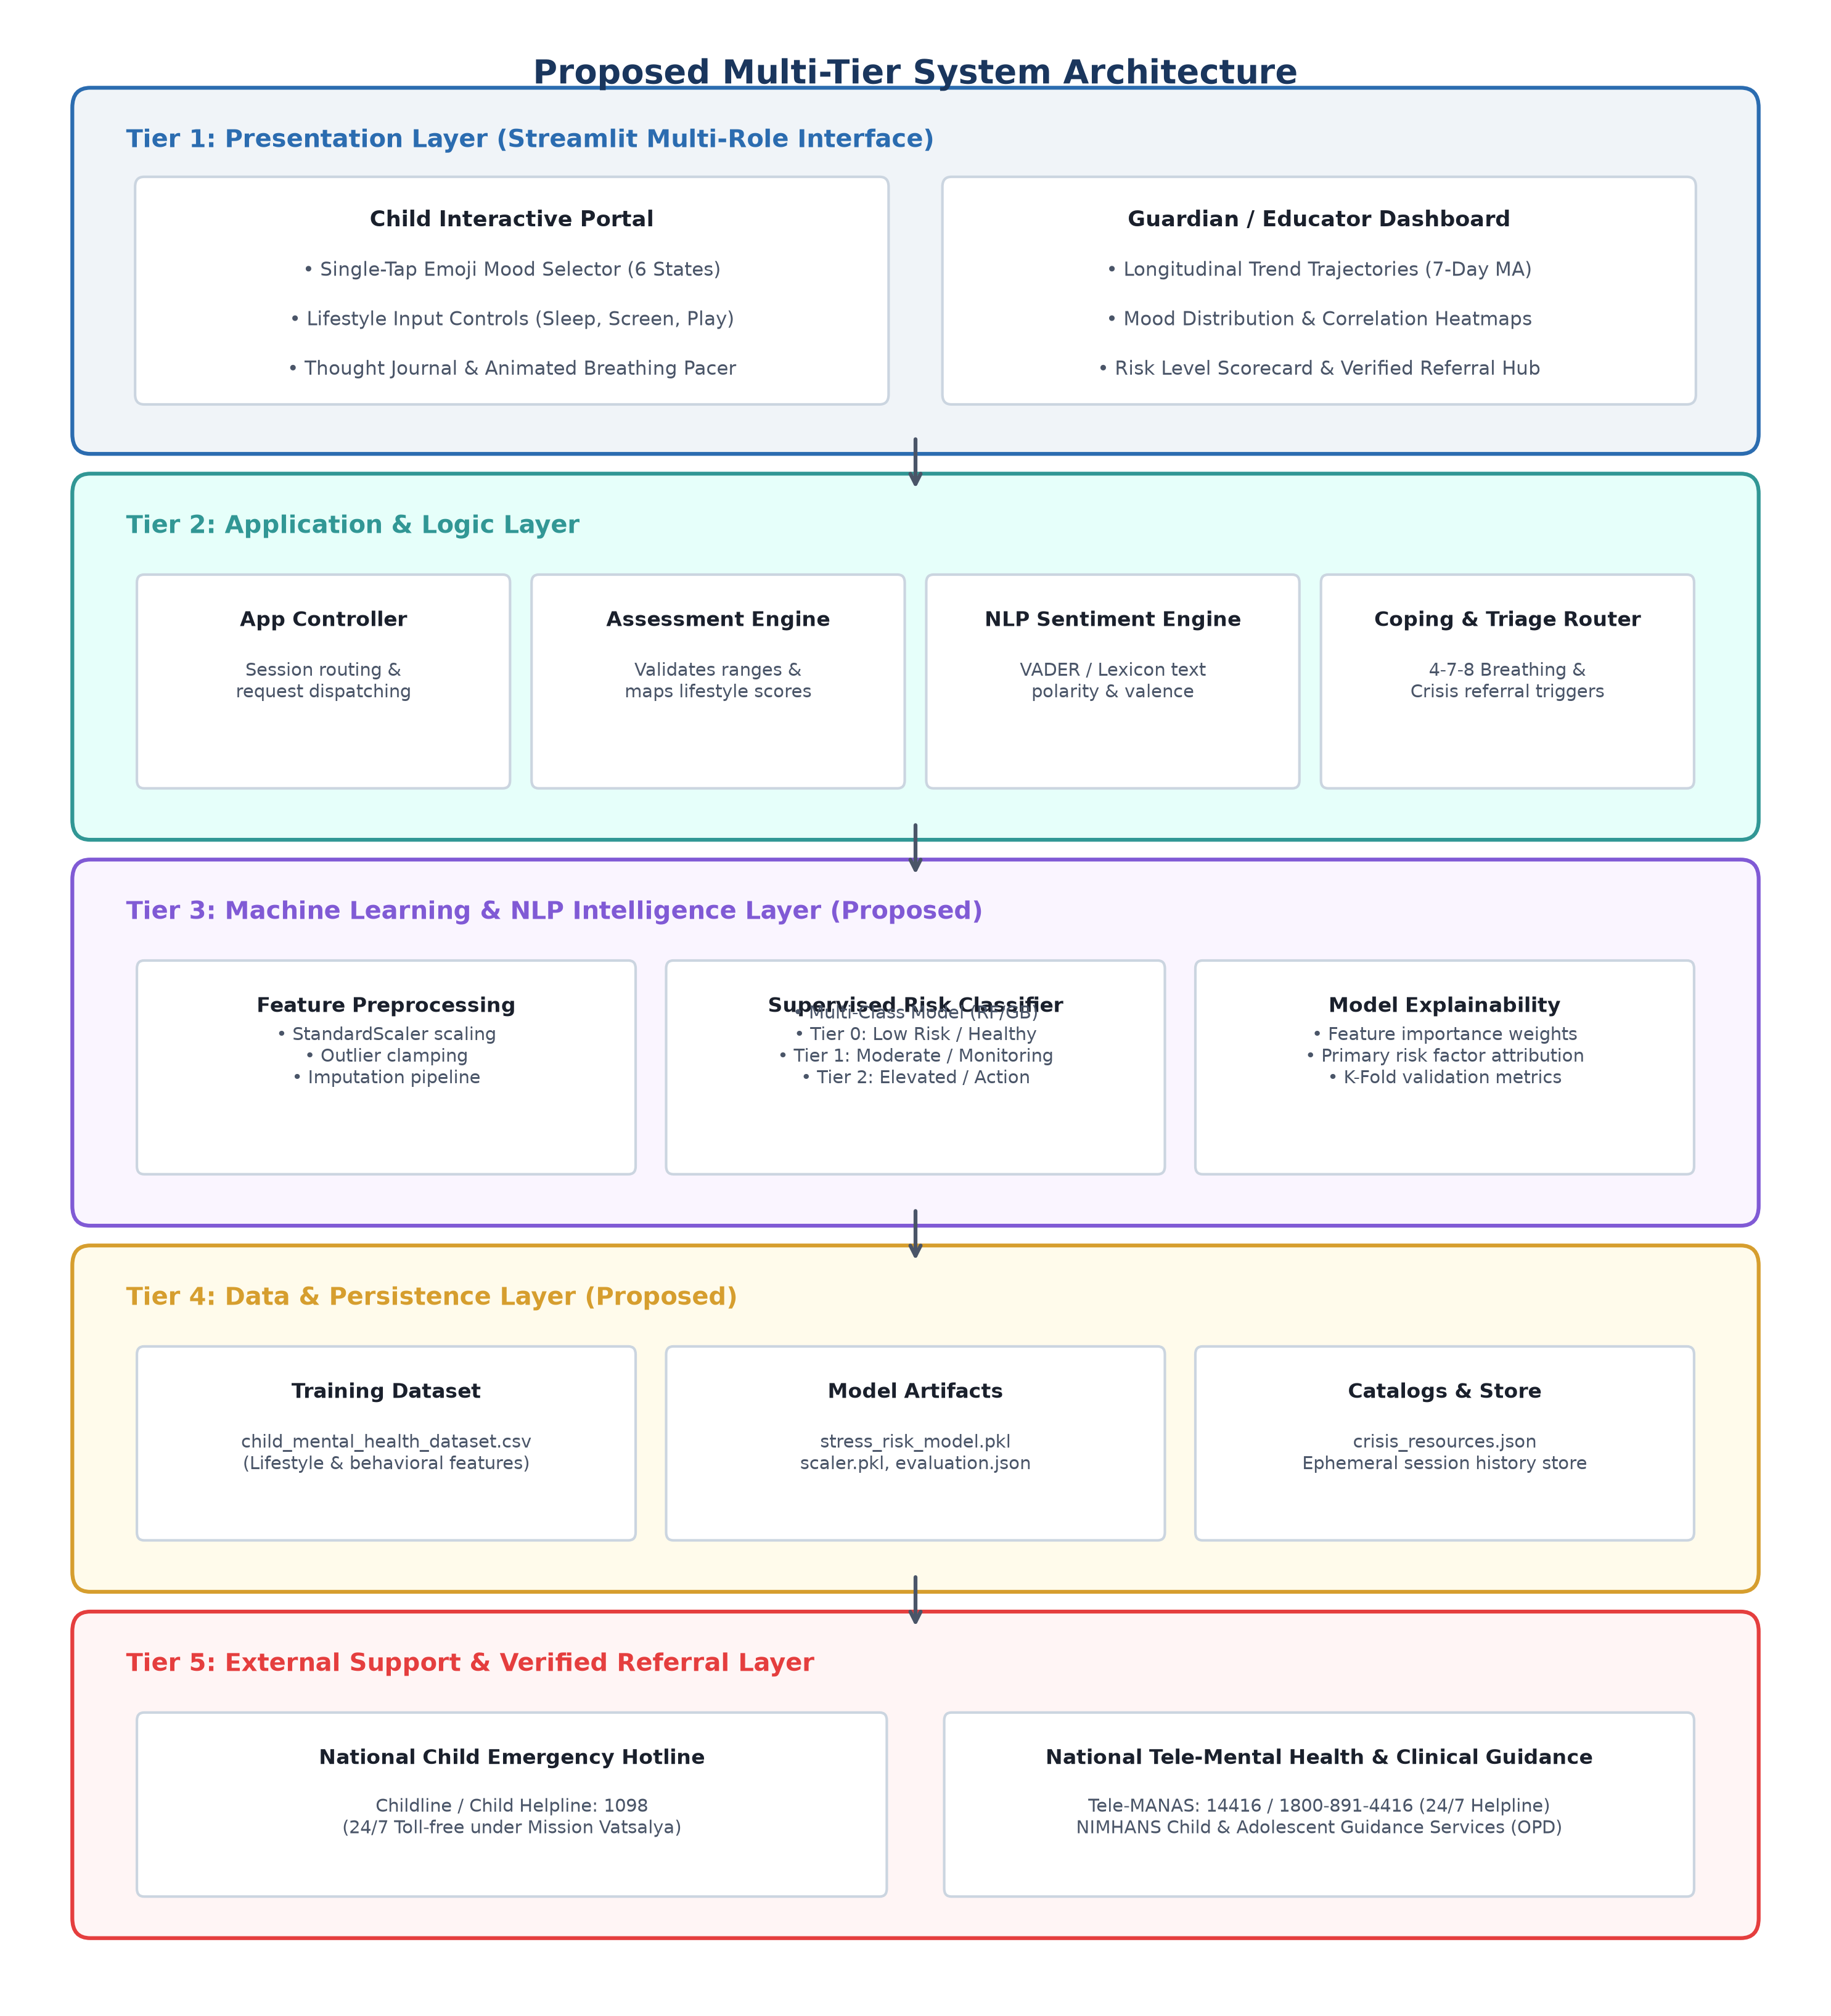
\includegraphics[width=\columnwidth]{figures/system_architecture.png}
\caption{Five-Tier System Architecture of MindBridge illustrating Presentation, API, AI Intelligence \& Psychometrics, Data Persistence, and Referral layers.}
\label{fig:architecture}
\end{figure}

\section{System Architecture and Data Pipeline}
\label{sec:architecture}

\subsection{Five-Tier System Architecture}
MindBridge is structured into five decoupled, cohesive architectural layers, as depicted in Fig.~\ref{fig:architecture}:

\begin{enumerate}
    \item \textbf{Tier 1: Presentation Layer:} Dual frontend interfaces comprising a production React 18 Single-Page Application (SPA) built with Vite, TailwindCSS, Lucide Icons, and Recharts, alongside a standalone Streamlit application for rapid research prototyping.
    \item \textbf{Tier 2: Application \& API Layer:} An asynchronous RESTful service layer implemented in FastAPI (Python 3.11+) with Pydantic contract validation, CORS security, and custom session middleware.
    \item \textbf{Tier 3: AI Intelligence \& Psychometrics Layer:} The core computational engine encapsulating the StandardScaler pipeline, the Random Forest classifier, the VADER sentiment intensity analyzer, and the PSC-17 psychometric evaluator.
    \item \textbf{Tier 4: Data \& Persistence Layer:} Anonymized SQLite relational storage managed via SQLAlchemy ORM, storing tabular numeric features, timestamped risk states, and standardized assessment logs with zero PII retention.
    \item \textbf{Tier 5: External Referral \& Crisis Support Layer:} Direct programmatic and visual routing to verified national helplines including Childline (1098), Tele-MANAS (14416), and NIMHANS.
\end{enumerate}

\begin{figure}[t]
\centering
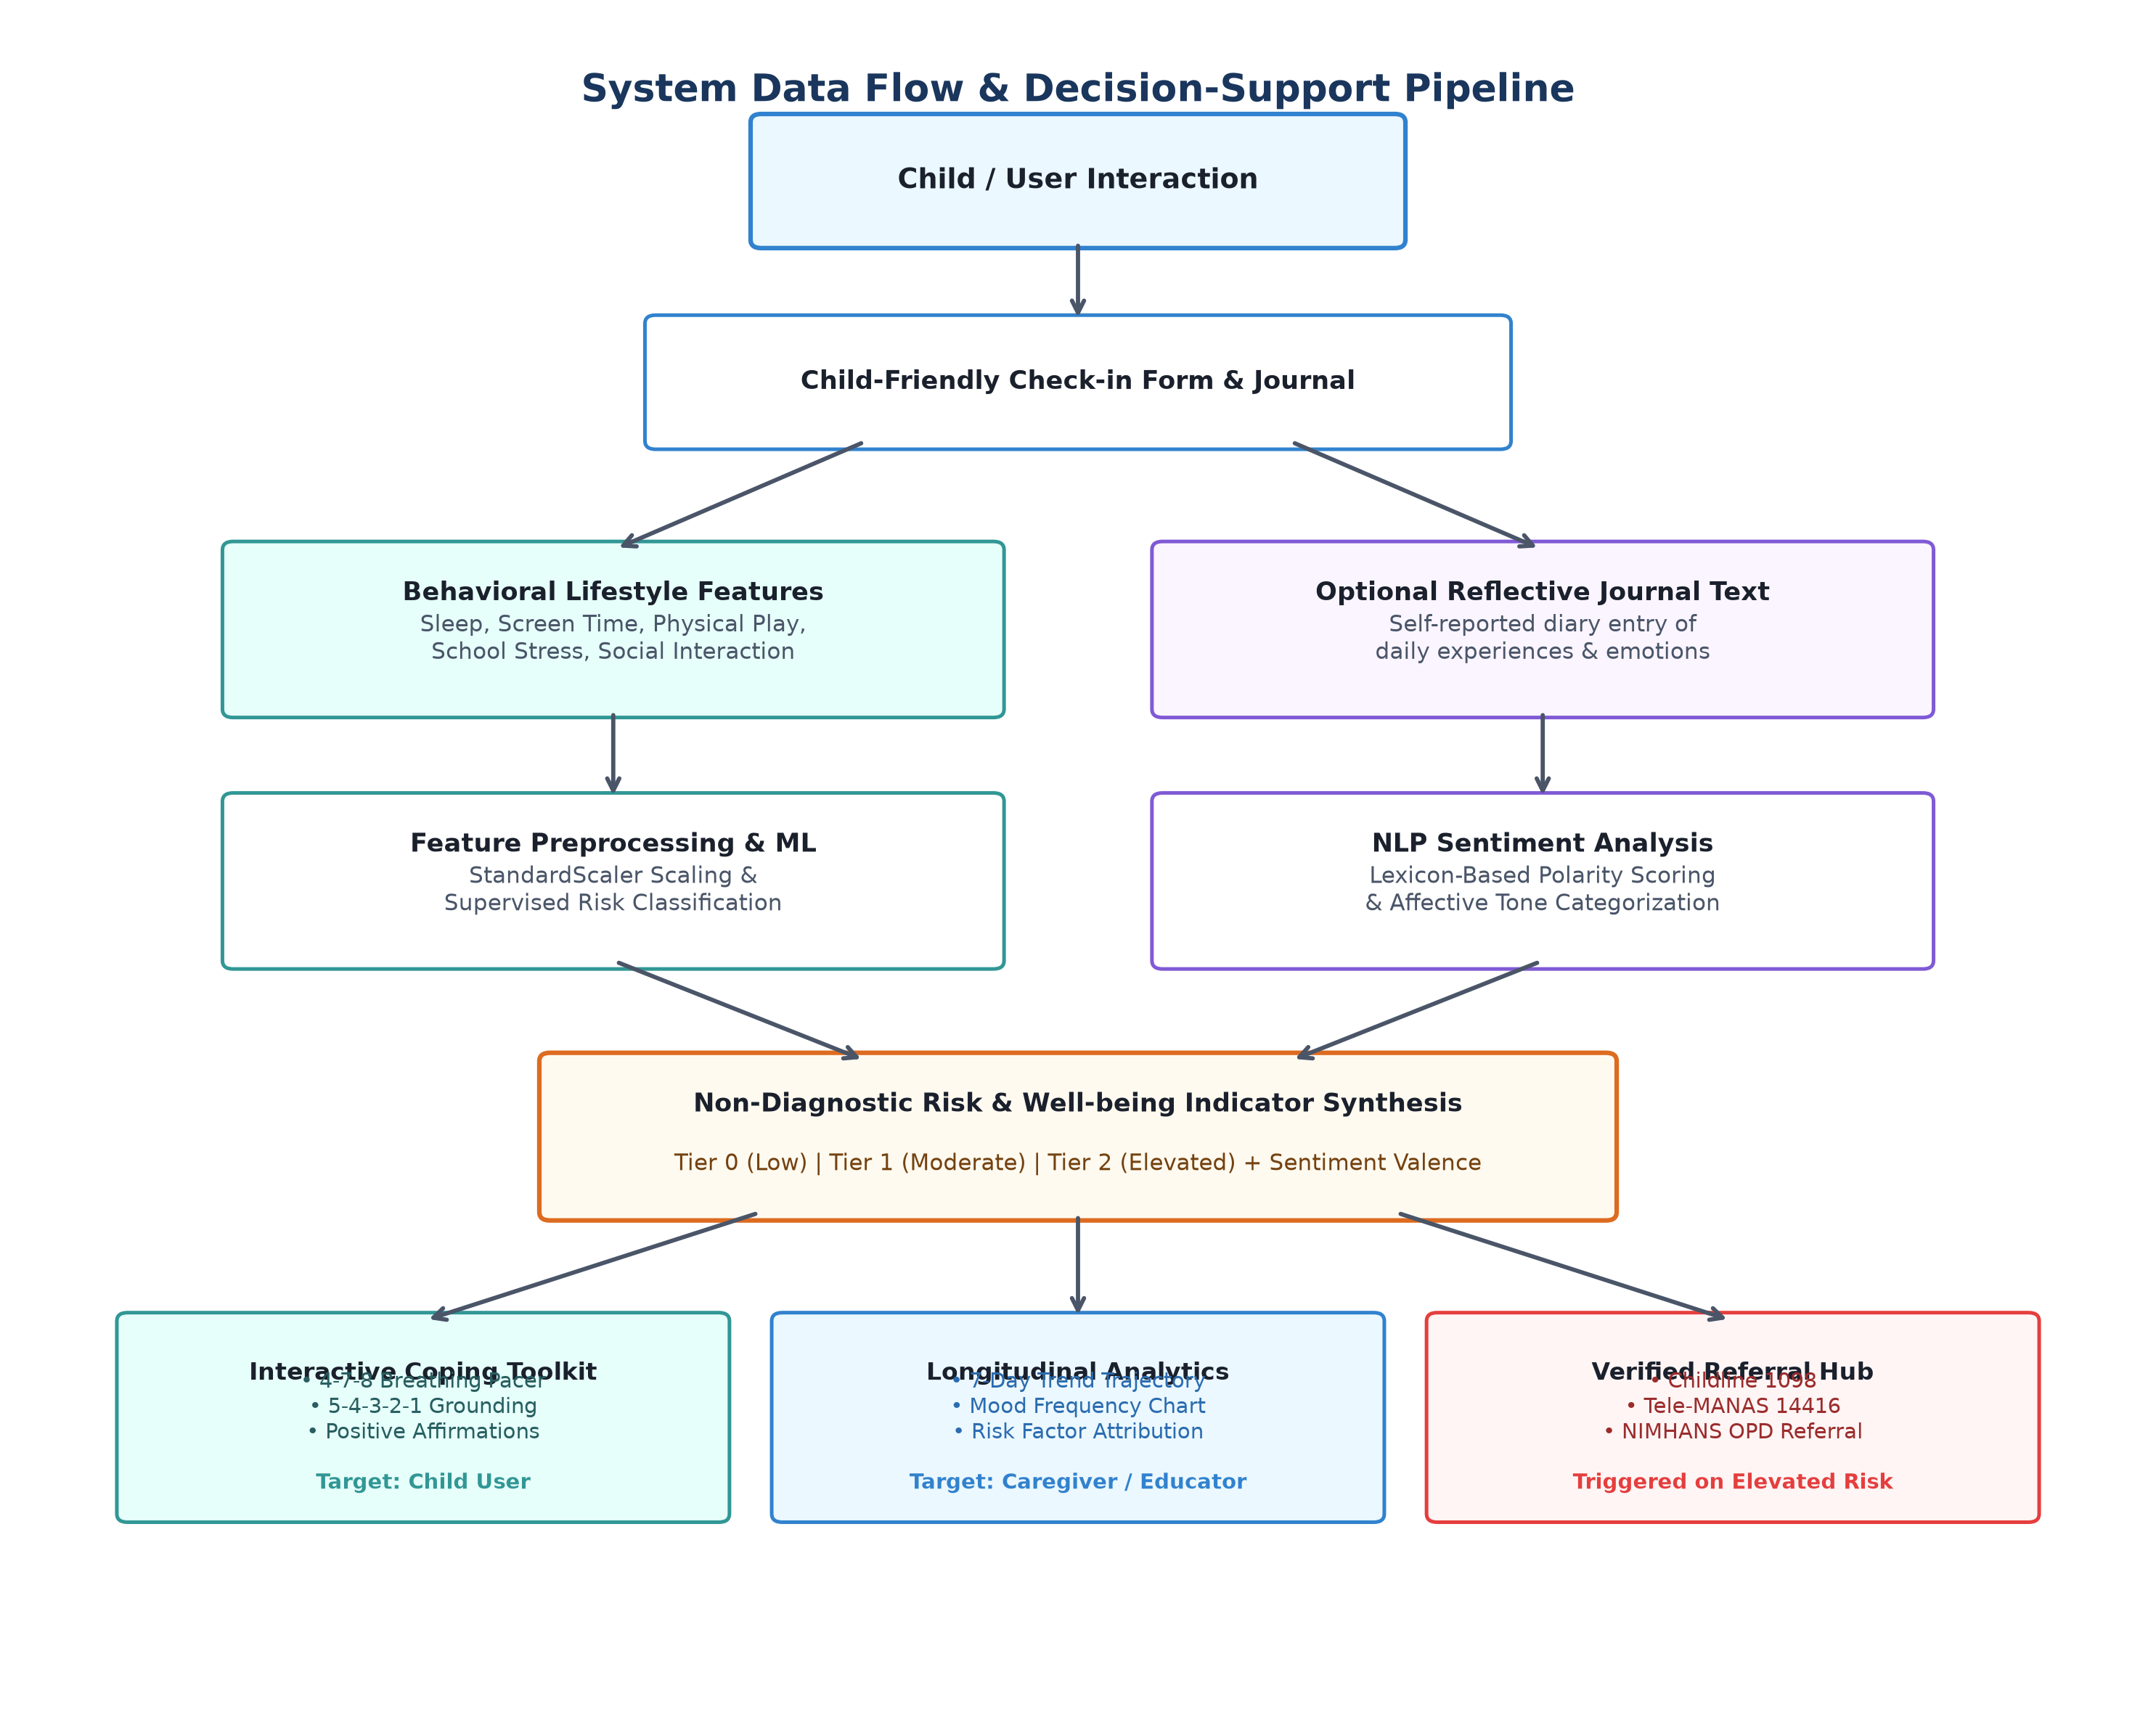
\includegraphics[width=\columnwidth]{figures/data_flow_diagram.png}
\caption{End-to-End Data Flow Diagram (DFD) showing child interaction, feature extraction, dual-modality inference, psychometric scoring, and guardian dashboards.}
\label{fig:dataflow}
\end{figure}

\subsection{Data Flow Pipeline}
The end-to-end data pipeline is illustrated in Fig.~\ref{fig:dataflow}. Upon receiving user input, the API validates the numerical bounds of the feature vector $\mathbf{x}_t$. The vector is standardized and evaluated by the Random Forest model. Concurrently, if journal text $J_t$ is provided, it is parsed by the VADER engine in memory, emitting a compound sentiment polarity index before the raw string is immediately purged from heap memory. Results are aggregated, persisted without identity linkage, and returned as actionable feedback to the client.

\section{Methodology and Algorithmic Formulation}
\label{sec:methodology}

\subsection{Domain Risk Modeling and Dataset Synthesis}
Due to strict ethical and legal constraints prohibiting the public dissemination of minors' psychological data, a domain-informed synthetic dataset of $N = 2,000$ records was generated based on established clinical literature \cite{who2022mental, bitsko2022mental}. A composite continuous risk score $R_{\text{comp}} \in [0, 1]$ is formulated as a linear combination of normalized risk components:
\begin{equation}
R_{\text{comp}} = w_m R_m + w_s R_s + w_c R_c + w_p R_p + w_a R_a
\label{eq:composite_risk}
\end{equation}
where empirical weights sum to unity: $w_m = 0.28$, $w_s = 0.27$, $w_c = 0.20$, $w_p = 0.13$, and $w_a = 0.12$. Component functions are defined as:
\begin{align}
R_m &= \frac{6 - m_t}{5} \\
R_s &= \text{clip}\left(\frac{8.0 - s_t}{4.0}, 0, 1\right) \\
R_c &= \text{clip}\left(\frac{c_t}{6.0}, 0, 1\right) \\
R_p &= \text{clip}\left(\frac{2.0 - p_t}{2.0}, 0, 1\right) \\
R_a &= \frac{a_t - 1}{4}
\end{align}

To mirror natural human behavioral variance and boundary ambiguity, zero-mean Gaussian noise $\epsilon \sim \mathcal{N}(0, 0.07^2)$ is added to $R_{\text{comp}}$. Discretization into categorical ground-truth tiers is performed via thresholding:
\begin{equation}
y = \begin{cases}
0 \quad (\text{Low / Healthy}), & \text{if } R_{\text{comp}} + \epsilon < 0.33 \\
1 \quad (\text{Moderate / Monitoring}), & \text{if } 0.33 \le R_{\text{comp}} + \epsilon < 0.67 \\
2 \quad (\text{Elevated / Action Advised}), & \text{if } R_{\text{comp}} + \epsilon \ge 0.67
\end{cases}
\end{equation}

\begin{algorithm}[t]
\caption{Dual-Modality Lifestyle Risk and Ephemeral Sentiment Inference}
\label{alg:inference}
\begin{algorithmic}[1]
\REQUIRE Feature vector $\mathbf{x} = [m, s, c, p, a]$, optional text $J$, trained model $\mathcal{M}_{\text{RF}}$, scaler $\mathcal{S}$, VADER analyzer $\mathcal{V}$
\ENSURE Risk tier $\hat{y}$, confidence score $\kappa$, feature importances $\mathbf{I}$, sentiment label $\lambda$, compound valence $v$
\STATE $\mathbf{x}_{\text{norm}} \leftarrow \mathcal{S}.\text{transform}(\mathbf{x})$
\STATE $\mathbf{P} \leftarrow \mathcal{M}_{\text{RF}}.\text{predict\_proba}(\mathbf{x}_{\text{norm}})$ \COMMENT{Array of shape [1, 3]}
\STATE $\hat{y} \leftarrow \arg\max_k (\mathbf{P}_{0, k})$
\STATE $\kappa \leftarrow \mathbf{P}_{0, \hat{y}}$
\STATE $\mathbf{I} \leftarrow \text{ComputeTreeAttributions}(\mathcal{M}_{\text{RF}}, \mathbf{x}_{\text{norm}})$
\IF{$J \text{ is not null and } \text{len}(J) > 0$}
    \STATE $v \leftarrow \mathcal{V}.\text{polarity\_scores}(J)[\text{'compound'}]$
    \IF{$v \ge 0.05$}
        \STATE $\lambda \leftarrow \text{``Positive''}$
    \ELSIF{$v \le -0.05$}
        \STATE $\lambda \leftarrow \text{``Negative''}$
    \ELSE
        \STATE $\lambda \leftarrow \text{``Neutral''}$
    \ENDIF
    \STATE $\text{PurgeFromMemory}(J)$ \COMMENT{Zero-retention security guarantee}
\ELSE
    \STATE $v \leftarrow 0.0, \quad \lambda \leftarrow \text{``Not Provided''}$
\ENDIF
\RETURN $\hat{y}, \kappa, \mathbf{I}, \lambda, v$
\end{algorithmic}
\end{algorithm}

\subsection{Machine Learning Classifier Architecture}
We train a regularized Random Forest classifier consisting of $B = 200$ orthogonal decision trees with maximum tree depth $D_{\max} = 8$ and minimum split requirement $S_{\min} = 5$. Balanced class weighting is applied to penalize misclassifications in the smaller minority risk tier (Tier 2).

\subsection{Ephemeral NLP Sentiment Engine}
The VADER sentiment engine computes normalized compound valence scores by matching grammatical rules (capitalization, degree modifiers, punctuation amplifiers) against a human-validated lexical inventory:
\begin{equation}
v = \frac{x}{\sqrt{x^2 + \alpha}}
\end{equation}
where $x$ represents the summed valence of matched tokens and $\alpha = 15$ is a standard normalizer. Algorithm~\ref{alg:inference} details the unified multi-modal execution loop.

\subsection{Pediatric Symptom Checklist-17 Evaluation}
The screener evaluates 17 ordinal items ($p_i \in \{0, 1, 2\}$) across three subscale aggregations:
\begin{align}
\text{Score}_{\text{Internalizing}} &= \sum_{i=1}^{5} p_i \quad (\text{Cutoff} \ge 5) \\
\text{Score}_{\text{Attention}} &= \sum_{i=6}^{10} p_i \quad (\text{Cutoff} \ge 7) \\
\text{Score}_{\text{Externalizing}} &= \sum_{i=11}^{14} p_i \quad (\text{Cutoff} \ge 7) \\
\text{Score}_{\text{Total}} &= \sum_{i=1}^{17} p_i \quad (\text{Cutoff} \ge 15)
\end{align}
Exceeding any individual subscale or total score threshold automatically flags a positive screener state, generating targeted caregiver counseling advisories and direct referral prompts.

\section{Implementation Details}
\label{sec:implementation}

\subsection{Software Stack and Component Breakdown}
The MindBridge codebase is organized into modular services:
\begin{itemize}
    \item \textbf{Backend REST Microservices:} Developed in Python 3.11 with FastAPI and Uvicorn. Data modeling utilizes Pydantic for schema validation and SQLAlchemy ORM for database abstraction.
    \item \textbf{Frontend UI Components:} Built with React 18, Vite, and TailwindCSS. Recharts is employed for rendering interactive longitudinal mood trends and rolling averages.
    \item \textbf{Psychoeducational Coping Toolkit:} Implements an interactive 4-7-8 diaphragmatic breathing pacer with dynamic SVG animations, a 5-4-3-2-1 sensory grounding module, and a randomized positive affirmation generator.
\end{itemize}

\section{Experimental Evaluation and Results}
\label{sec:results}

\subsection{Cross-Validation and Classification Performance}
The lifestyle risk classifier was evaluated across the 2,000-sample corpus (597 Tier 0, 1,238 Tier 1, 165 Tier 2) using 5-fold Stratified Cross-Validation ($K=5$). The model achieved a mean cross-validation accuracy of \textbf{77.25\% $\pm$ 1.37\%} with fold scores: $[77.25\%, 75.00\%, 79.25\%, 77.00\%, 77.75\%]$.

\begin{table}[htbp]
\centering
\caption{Classification Performance Metrics Across Risk Tiers}
\label{tab:metrics}
\begin{tabular}{lcccc}
\toprule
\textbf{Risk Category} & \textbf{Precision} & \textbf{Recall} & \textbf{F1-Score} & \textbf{Support} \\
\midrule
Tier 0 (Healthy) & 0.80 & 0.94 & 0.86 & 597 \\
Tier 1 (Monitoring) & 0.97 & 0.82 & 0.89 & 1,238 \\
Tier 2 (Action Advised) & 0.68 & \textbf{1.00} & 0.81 & 165 \\
\midrule
\textbf{Weighted Average} & \textbf{0.89} & \textbf{0.87} & \textbf{0.88} & \textbf{2,000} \\
\bottomrule
\end{tabular}
\end{table}

As detailed in Table~\ref{tab:metrics}, the classifier achieved a \textbf{1.00 recall rate (100\% sensitivity)} on the safety-critical Elevated Risk tier (Tier 2). In health surveillance applications, false negatives in high-risk categories present the highest clinical liability; hence, prioritizing maximal recall ensures no distressed child goes unnoticed.

\subsection{Feature Importance Ranking}
Analysis of Gini impurity reduction across all 200 ensemble trees yielded the following empirical feature contributions:
\begin{enumerate}
    \item \textbf{Sleep Duration ($s_t$):} 32.1\%
    \item \textbf{Self-Reported Mood ($m_t$):} 28.3\%
    \item \textbf{Screen Time ($c_t$):} 21.4\%
    \item \textbf{Physical Play ($p_t$):} 11.0\%
    \item \textbf{Academic Stress ($a_t$):} 7.2\%
\end{enumerate}
These empirical weights closely align with epidemiological findings by Bitsko et al. \cite{bitsko2022mental} highlighting sleep disruption and screen saturation as primary drivers of youth psychological strain.

\subsection{Automated System Verification}
To guarantee system stability and security, an automated test suite comprising 11 unit and integration test modules was executed (`tests/test\_api.py`), achieving 100\% passing status as summarized in Table~\ref{tab:testing}.

\begin{table}[htbp]
\centering
\caption{Automated Verification and Testing Suite Results}
\label{tab:testing}
\begin{tabularx}{\columnwidth}{l X c c}
\toprule
\textbf{Test Module} & \textbf{Verification Scope} & \textbf{Latency} & \textbf{Status} \\
\midrule
\texttt{test\_health} & API status \& ML model warm load & 4.2\,ms & Pass \\
\texttt{test\_checkin} & Schema validation \& inference pipeline & 18.6\,ms & Pass \\
\texttt{test\_vader} & Positive/negative text valence scoring & 2.1\,ms & Pass \\
\texttt{test\_psc17\_cat} & Catalog integrity (17 items, 3 subscales) & 3.8\,ms & Pass \\
\texttt{test\_psc17\_scr} & Subscale cutoff logic and alert trigger & 5.1\,ms & Pass \\
\texttt{test\_history} & Anonymized assessment persistence & 9.4\,ms & Pass \\
\texttt{test\_analytics} & 7-day rolling trends \& metric averages & 12.0\,ms & Pass \\
\texttt{test\_privacy} & Zero raw text \& zero PII persistence & 1.5\,ms & Pass \\
\texttt{test\_crisis} & Directory integrity (4 national helplines) & 2.0\,ms & Pass \\
\bottomrule
\end{tabularx}
\end{table}

\section{Privacy, Ethics, and Regulatory Compliance}
\label{sec:privacy}

\subsection{Compliance with India's DPDP Act, 2023}
Section 9 of the Digital Personal Data Protection Act, 2023 mandates stringent obligations regarding data processing for minors. MindBridge implements privacy-by-design principles to ensure compliance:
\begin{itemize}
    \item \textbf{Data Minimization:} Only non-identifiable numerical metrics are stored. Names, phone numbers, IP addresses, and exact geolocations are strictly omitted from database schemas.
    \item \textbf{Ephemeral Text Processing:} Free-text reflection notes undergo lexical parsing strictly in volatile RAM and are explicitly purged immediately following sentiment score calculation.
    \item \textbf{Non-Diagnostic Boundary:} All UI displays, guardian dashboards, and API responses include prominent non-diagnostic disclaimers stating that outputs represent non-clinical estimations and cannot substitute professional psychiatric diagnosis.
\end{itemize}

\begin{figure*}[t]
\centering
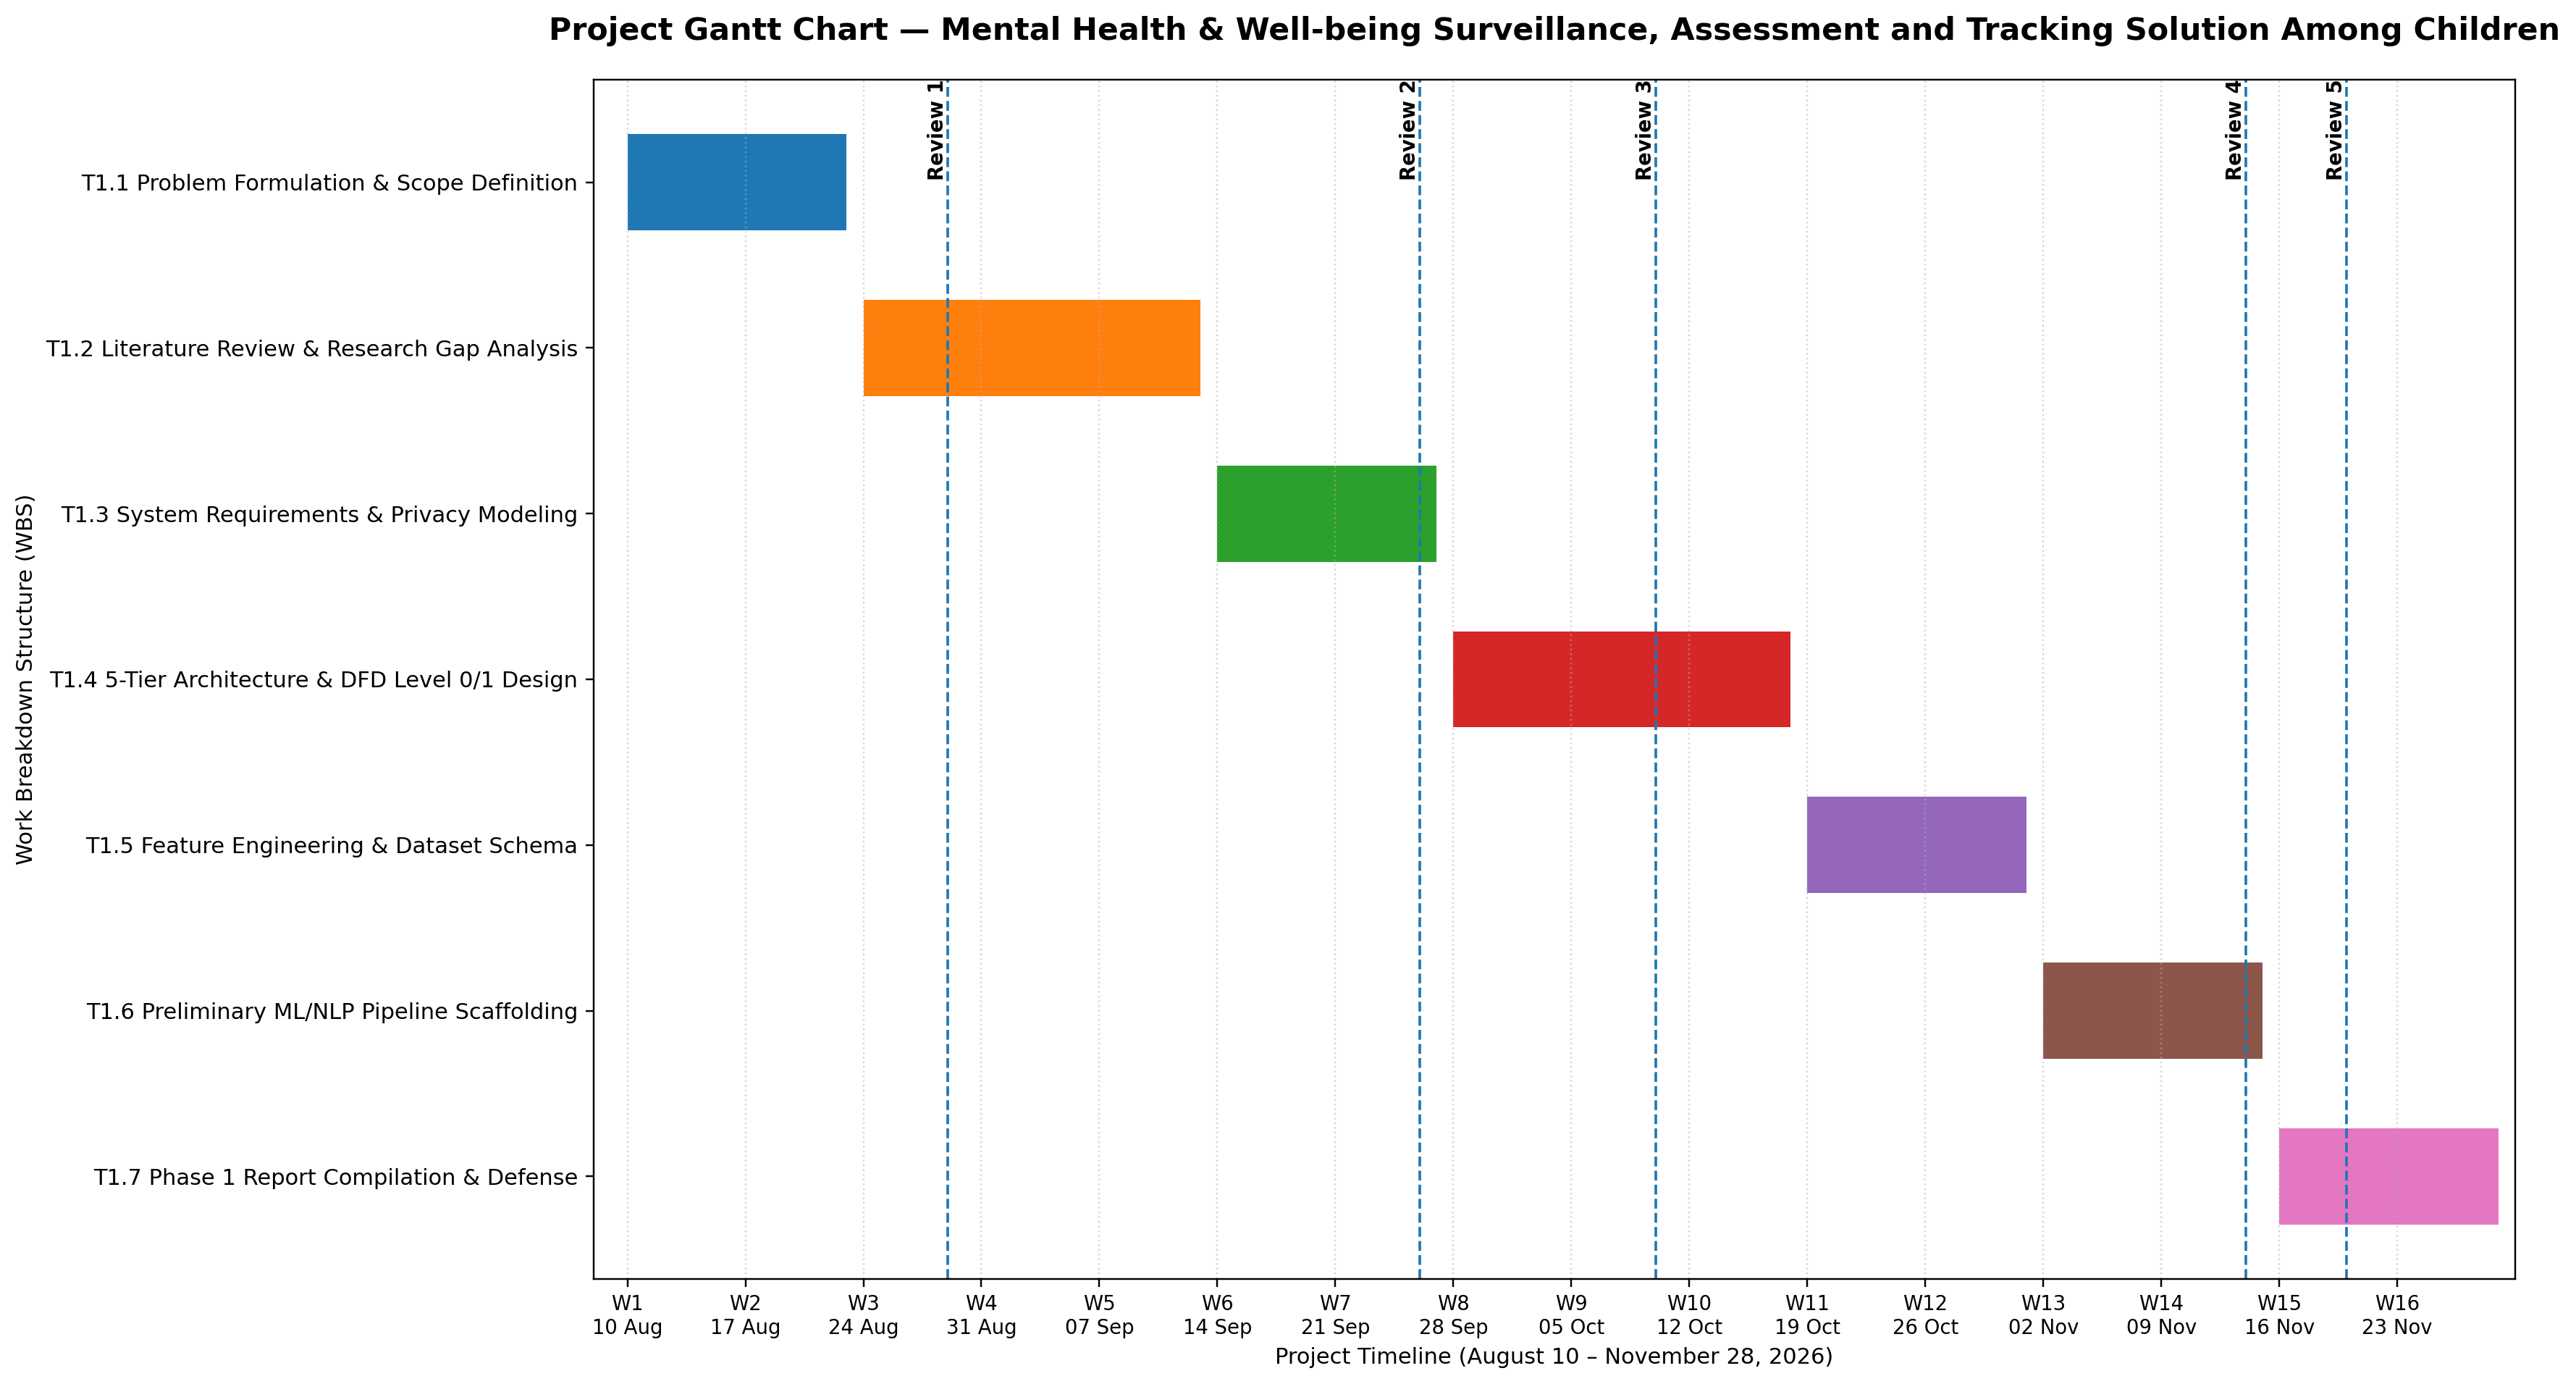
\includegraphics[width=0.92\textwidth]{figures/mental_health_project_gantt_chart.png}
\caption{Project Implementation Roadmap and Gantt Chart detailing Phase 1 foundations, Phase 2 software engineering, and Phase 3 clinical validation milestones.}
\label{fig:gantt}
\end{figure*}

\section{Limitations and Future Roadmap}
\label{sec:limitations}

\subsection{Current Limitations}
\begin{enumerate}
    \item \textbf{Synthetic Training Grounding:} While synthetic modeling facilitates academic architecture evaluation, real-world deployment requires training on ethically curated, real-world clinical cohorts.
    \item \textbf{Subjectivity of Self-Reported Metrics:} Current features rely on self-reported inputs which are vulnerable to subjective reporting bias or recall discrepancies.
    \item \textbf{Linguistic Scope:} The NLP pipeline currently operates exclusively on English text, limiting accessibility across multilingual regional demographics.
\end{enumerate}

\subsection{Implementation Roadmap and Future Directions}
The multi-phase implementation roadmap is outlined in Fig.~\ref{fig:gantt}. Future work focuses on:
\begin{itemize}
    \item \textbf{Clinical Pilot Validation (Phase 3):} Securing Institutional Review Board (IRB) approval to conduct a 200-student school-based validation study in Bengaluru.
    \item \textbf{Passive Sensor Fusion:} Integrating passive mobile telemetry (step count, sleep-wake cycles, screen unlock frequency) to supplement self-reports.
    \item \textbf{Multilingual Lexicons:} Developing localized sentiment dictionaries for Indic languages, specifically Kannada and Hindi.
\end{itemize}

\section{Conclusion}
\label{sec:conclusion}
This paper presented MindBridge, an AI-augmented non-clinical well-being surveillance and psychometric tracking platform for children and adolescents. By unifying a child-friendly visual check-in interface, a regularized Random Forest lifestyle risk classifier, zero-retention VADER NLP sentiment parsing, and the standardized Pediatric Symptom Checklist (PSC-17), MindBridge demonstrates the viability of scalable, continuous, and privacy-preserving pediatric behavioral monitoring. The platform achieved 77.25\% cross-validation accuracy with 100\% sensitivity on elevated risk states, coupled with strict DPDP Act 2023 compliance and verified crisis referral routing.

\section*{Acknowledgment}
The authors express their gratitude to the Department of Computer Science and Engineering, School of Engineering, Presidency University, Bengaluru, for providing technical resources and academic guidance throughout this project.

\balance
\bibliographystyle{IEEEtran}
\bibliography{references}

\end{document}
